% !TEX TS-program = pdflatex
% !TeX spellcheck = en_GB

\documentclass[11pt]{article}
%\overfullrule=1mm
\usepackage[T1]{fontenc}
\usepackage{lmodern}
\usepackage{fullpage}
%\usepackage{geometry}                % See geometry.pdf to learn the layout options. There are lots.
%\geometry{a4paper}                   % ... or a4paper or a5paper or ...
%\geometry{landscape}                % Activate for for rotated page geometry
%\usepackage[parfill]{parskip}    % Activate to begin paragraphs with an empty line rather than an indent
\usepackage{graphicx}
\usepackage{DotArrow}
\usepackage{hyperref}
\usepackage{listings}
\lstset{basicstyle=\small}

%\usepackage{amsfonts}
%\usepackage{fancyhdr}
%\usepackage{cite}
%\usepackage{ifthen}
%\usepackage{amssymb}
%\usepackage{fancyhdr}
%\usepackage{pifont}
\usepackage{stmaryrd}
\usepackage{mathtools,mathpartir}
\usepackage{proof}
%\usepackage{setspace}
%\usepackage{indentfirst}
\usepackage{amsmath,amssymb,amscd,mathrsfs}
\DeclareGraphicsRule{.tif}{png}{.png}{`convert #1 `dirname #1`/`basename #1 .tif`.png}
\usepackage{epsfig,color,subfigure,enumitem,soul}
\newcommand{\TODO}[1]{\textcolor{red}{\textbf{[TODO:#1]}}}
\newcommand{\NOTE}[1]{\textcolor{blue}{\textbf{[NOTE:#1]}}}
\newcommand{\ERIC}[1]{\textcolor{blue}{#1}}
\definecolor{darkgreen}{rgb}{0.1, 0.5, 0.1}
\newcommand{\LUDO}[1]{\textcolor{darkgreen}{#1}}
\newcommand{\RAB}[1]{\textcolor{magenta}{#1}}
\newcommand{\coloncolon}{{:\hspace{-.2ex}:}}
\newcommand{\bigcupdot}{\charfusion[\mathop]{\bigcup}{\cdot}}
\makeatletter
\newcommand{\raisemath}[1]{\mathpalette{\raisem@th{#1}}}
\newcommand{\raisem@th}[3]{\raisebox{#1}{$#2#3$}}
\makeatother
\newcommand{\shortotimes}{\!\otimes\!}
\usepackage{macrospNets}

\newcommand{\nounderline}[1]{#1}


%\usepackage[math]{cellspace}
%\setlength\cellspacetoplimit{ 37pt}
%\setlength\cellspacebottomlimit{18pt}

%\pagestyle{plain}

% addition to the mathpartir package for red dotted rules,
% that we use for open-transitions


\newtheorem{theorem}{Theorem}
%\newtheorem{prop}{Proposition}
%\newtheorem{corollary}[theorem]{Corollary}
\newtheorem{lemma}{Lemma}
\newtheorem{algorithm}[theorem]{Algorithm}
%\newtheorem{remark}[theorem]{Remark}
\newtheorem{definition}{Definition}
\newtheorem{property}{Property}
\newtheorem{example}{Example}
%\newtheorem{problem}[theorem]{Problem}
%\newenvironment{proof}{\paragraph{Proof}}{}

\begin{document}

\title{ Open pNets
%\thanks{This work was partially funded by the Associated Team FM4CPS
%  between INRIA and ECNU, Shanghai}
}





\maketitle
%
%\section*{Status and TODO list}
%
%TODOS: AVRIL 2019
%
%- exemple (Eric: failure buffer)
%- biblio (rabea)
%- inuitions de preuves et intuition de bisim de cloture, etc. (Ludo)
%
%%% \TODO{voisr si on redefinit les bigotimes pour prendre des maps et retourner des maps au lieu des substitutions (et on englobe dans une subst a la fin)}
%
%%% \TODO{prendre soin des posts sur les actions partout}
%
%%% ===> dealine 14 Juillet
%
%%% TODOs du 19 decembre
%
%
%
%%% - enlever 5.2 et citer avocs
%
%%% - ajouter des proof sketch dans le papier
%
%%% - def 11 point 2:
%%% A, Pred, Post
%%% -----------   in T
%%% s->s'
%%% et A(j)=tau
%%% implies blablabla
%
%
%%% OLD OLD OLD (check)
%%% Notes de reunion 24 Sept
%
%
%%% - etat de l art: il faudrait des refs sur bisim en gemneral, probablement avec pas mal de pi calcul (Eric?), des refs sur pourquoi pnets et des refs sur utilite de la weak bisim en verif
%
%
%
%%% - target: JLamp
%
%%% Conventions
%%% [14/9/2018] 
%
%%% Dans le texte pas de $\backslash$ devant pNet et pLTS
%
%%% pNet devient P ou Q dans les equations; on garde $pLTS$
%
%%% \medskip
%
%%% TODOS et deadline
%
%
%%% Global and questions:
%%% \begin{itemize}
%%% \item \TODO{should we use iff/implies or LeftRightArrow/Rightarrow}
%%% \item related works
%%% \end{itemize}
%%% Ludo:
%%% \begin{itemize}
%%% \item[X] reorga sec weak bisim + thm -> 10 Juil
%%% \item[X]  intro et orga globale du papier -> fin aout
%%% \item[partial] explication dans semantique open pnets et composition
%%% \item uniformisation pNet P Q
%%% \end{itemize}
%
%



% \tableofcontents



\section{Background and notations}\label{sec:notations}
This section introduces the notations we will use in this article, and  recalls the definition of pNets~\cite{henrio:Forte2016} with an informal semantics  of the pNet constructs. The only significant difference compared to our previous definitions is that we remove here the restriction that was stating that variables should be local to a state of a labelled transition system.




\subsection{Notations}
%In general $x_i,y_i$ range over variables.
\subsubsection*{Term algebra.}
Our models rely on a notion of parameterised actions, that are
symbolic expressions using data types and variables. As our model aims
at encoding the low-level behaviour of possibly very different
programming languages, we do not want to impose one specific algebra
for denoting actions, nor any specific communication mechanism. So we
leave unspecified the constructors of the algebra that will allow building
expressions and actions. Moreover, we use a generic {\em action interaction}
mechanism, based on (some sort of) unification between two or more action
expressions, to express various kinds of communication or
synchronisation mechanisms.

%\def\Talg{\mathcal{T}_{\Sigma}}
%\def\BoolExprs{\mathcal{B}}
%\def\Exprs{\mathcal{E}} \TODO{use Exprs}
%\def\Actionalg{\mathcal{A}}

Formally, we assume the existence of a term algebra $\AlgT$,
where $\Sigma$ is the signature of the data and action constructors. Within $\AlgT$, we distinguish a set of
 expressions $\AlgE$, including a set of boolean
expressions $\AlgE$ ($\AlgB\subseteq\AlgE$). 
On top of $\AlgE$ we build the action algebra
$\AlgA$, with $\AlgA\subseteq\AlgT,
\AlgE\cap\AlgA=\emptyset$;
naturally action terms will use data expressions as sub-terms.
The function
$\vars(t)$ identifies the set of variables in a term
$t\in\AlgT$.

We let $e_i$ range over expressions ($e_i\in\AlgE$), $a$
range over action labels, $\symb{op}$ be operators, and $x_i$ and $y_i$ range over
variable names. 

We distinguish two kinds of parameterised actions: one that distinguishes input variables and one that does not. 
We first define the set of actions that distinguish input variables, they will be used in the definition of \pLTS\ below:
\[
\begin{array}[l]{rcl@{\quad}p{7.5cm}}
  \alpha\in\AlgA&::=&a(p_1,\ldots,p_n)&\text{action terms}\\
  p_i&::=& ?x~|~e_i&\text{parameters (input variable or expression)}\\
  e_i&::=& \symb{Value}~|~x~|~\symb{op}(\symb{e}_1,..,\symb{e}_n)&\text{Expressions}
\end{array}
\]
The \emph{input variables} in an action term are those marked with a
$\symb{?}$.
We additionally suppose that each input variable does not
appear somewhere else in the same action term:
$p_i=?x\Rightarrow\forall j\neq i.\, x\notin \vars(p_j)$.
We define $iv(t)$  as the set of input variables of a term $t$ (without the '?' marker).
Action algebras can encode naturally usual point-to-point message passing calculi (using 
$a(?x_1,...,?x_n)$ for inputs, $a(v_1,..,v_n)$ for outputs), but it also allows
for more general synchronisation mechanisms, like gate negociation in Lotos, or broadcast
communications. 

The set of actions that do not distinguish input variables is denoted $\AlgAS$, it will be used in synchronisation vectors of pNets:
\[\begin{array}[l]{rcl@{\quad}l}
  \alpha\in \AlgAS &::=&a(e_1,\ldots,e_n)
\end{array}
\]






\subsubsection*{Indexed sets}



In this article, we extensively use indexed structures 
(maps) over some countable indexed sets.   The indices can typically be
integers, bounded or not. We use indexed sets in pNets because we want to consider a set of processes, and specify separately how to synchronise them. Roughly this could also be realised using tuples, however indexed sets are more general, can be infinite, and give a compact representation than using the position in a possibly long tuple.

An indexed family is denoted as
follows: $a_i^{i\in I}$ is a family of elements $a_i$ indexed over the
set $I$. Such a family
is equivalent to the mapping $(i\mapsto a_i)^{i\in I}$, and we will also use mapping 
notations to manipulate indexed sets.
To specify the set over which the structure is indexed, 
indexed structures are always denoted with an exponent of the form $i\in I$.

Consequently, $a_i^{i\in I}$ defines first $I$ the set over which the
family is indexed, and then $a_i$ the elements of the family.
For example $a^{i\in\{3\}}$ is
the mapping with a single entry $a$ at index $3$; exceptionally, such mappings with
only a few entries will also be denoted $(3\mapsto a)$.
%The operation  $A[j \mapsto a]$ updates the value associated to $j$ in map $A$ so that 
%it 
%now corresponds to $a$. 

When this is not ambiguous, we shall use abusive vocabulary and
notations for sets, and typically write ``indexed set over I'' when  
formally we should speak of multisets, and ``$x\in
A_i^{i\in I}$'' to mean $\exists i\in I.\, x=A_i$.
%An empty family is denoted $[]$. % (it can be defined as $a_i^{i\in\emptyset}$).
To simplify equations, an indexed set can be denoted $\set{a}$
instead of $a_i^{i\in I}$ when $I$ is irrelevant.

$\uplus$ is the disjoint union on sets. We extend it to  disjoint union  of indexed 
sets defined by the merge of the 
two sets provided they are indexed on disjoint families.
The elements
of the union of two indexed sets are then accessed by using an index of one of the two
joined families.
%We suppose here that disjoint unions are always well defined; this
%requires to choose disjoint  
%indices in the definition of the component system (e.g. name of
%methods of different interfaces).
$\setminus$ is the standard subtraction operation on indexed sets: $\dom(A\setminus B)=\dom(A)\setminus B$.

%%\smallskip\noindent
%\paragraph*{Indexed sets.}
%We extensively use indexed structures
%over some countable indexed sets, which are equivalent to mappings over
%the countable set. % . The indexes will usually be
%% integers, bounded or not. Such an indexed family is
%%denoted
%%follows:
%$a_i^{i\in I}$
%%, or equivalently  $(i\mapsto a_i)^{i\in I}$
%denotes a family of elements $a_i$ indexed over the
%set $I$. % Such a family
%% is equivalent to the mapping $(i\mapsto a_i)^{i\in I}$.
%% To specify the set over which the structure is indexed,
%% indexed structures are always denoted with an exponent of the form $i\in I$
%% (arithmetic only appears in the indexes if necessary).
%$a_i^{i\in I}$ defines both $I$ the set over which the family is
%indexed (called \emph{range}), and $a_i$ the elements of the family.
%E.g., $a^{i\in\{3\}}$ is the mapping with a single entry $a$ at index
%$3$ ; abbreviated $(3\mapsto a)$ in the following.
%When this is not
%ambiguous, we shall use notations for sets, and typically write
%``indexed set over I'' when formally we should speak of multisets, and
%write $x\in a_i^{i\in I}$ to mean $\exists i\in I.\, x=a_i$.  An empty
%family is denoted $\emptyset$. We
%denote classically with an overline -- $\set{a}$  -- a family when the indexing set 
%is
%not meaningful.  $\uplus$ is the disjoint union on
%indexed sets.


\subsubsection*{Substitutions}
\label{def:substitutions}

We denote $y\gets e$ a substitution. The application of the substitution is denoted
$\subst{y\gets e}$, the operation replaces in a term all occurrences 
of the variable $y$ by the expression $e$. 
$\Post$ ranges over (indexed) sets of substitutions; $\subst{\Post}$ is the substitution that applies all the substitutions defined by $\Post$ in a parallel manner. $\otimes$ is the composition operator on substitutions, such that for any term $t$ we have: $t\subst{\Post\shortotimes\Post'} = (t\subst{\Post'})\subst{\Post}$.

For this property to be valid even if the substitution does not operate on all variables,
we define the composition operation as follows: 

\[(x_{k}\gets e_{k})^{k\in K}\shortotimes (x'_{k'}\gets e'_{k'})^{k'\in K'} =  
(x_{k}\gets e_{k}\subst{(x'_{k'}\gets e'_{k'})^{k'\in K'}})^{k\in K} \cup (x'_{k'}\gets e'_{k'})^{k'\in K''}\]
where $K''=\{k'\in K'|x'_{k'}\not\in\{x_k\}^{k\in K}\}$


\section{A model of process composition}\label{sec:OT}

The semantics of open pNets will be defined  as an open automaton. An open
automaton is an automaton where each transition composes transitions of several LTSs with
action of some holes, the transition occurs if some predicates hold, and can involve a 
set of state modifications. This section defines open automata and a bisimulation theory for them. This section can be viewed as an improved version of the formalism described in \cite{henrio:Forte2016}, extending the automata with a notion of global variable, which makes the state of the automaton more explicit. We also adopt a semantics and logical interpretation of the automata that intuitively can be stated as follows: ``if a transition belongs to an open automaton, any refinement of this transition also belongs to the automaton''.

\subsection{Open Automata}
 Open automata (OA) are not composition structures but they are made of transitions that are dependent of the actions of the holes, and they can reason on a set of variables (potentially with only symbolic values). 
%\TODO{adopt a uniform notation for open transitions, almost each instance has a 
%different 
%notation! I suggest p,l,pr,po using \{\} for p,l,po as they are sets}
\begin{definition}[Open transitions]\label{def:OT}
	\label{def:OpenTransitions}
	An \emph{open transition} (OT) over a
	set $J$ of holes with sorts $\Sort_j^{j\in J}$, a set $V$ of variables, and a set of states $\mathcal{S}$ is 
	a structure of the form:	
	\begin{mathpar}
	\openrule
	{	\beta_j^{j\in J'}, \Pred, \phi}
	{s \OTarrow {\alpha}s'}
	\end{mathpar}
	Where $J'\subseteq J$, $s, s'\in\mathcal{S}$ and $\beta_j$
        is a transition of the hole $j$, with $\beta_j\in\Sort_j$. 
Let $W$ be the set of variables in $V$ and all variables
        in the different terms
       $\beta_j$ and $\alpha$.
$\alpha$ is an action 
        label denoting the resulting action of this open transition.
        \Pred\ is a predicate over the set of variables $W$. $\phi$, called \emph{effect} is a mapping from variables in $V$ to expressions over the set of variables $W$. $V$ is called the domain of the effect.
 Open transitions are identified
        modulo logical equivalence on their predicate. 
\end{definition}

It is important to understand the difference between the red dotted rule and a normal 
inference rule. They correspond to two different logical levels.
On one side, classical (black) inference rules  use  an expressive logic and are paper rules.
 On the other side, open transition rules (with dotted lines) are logical implications, but using a simple logic (this logic includes the boolean expressions $\AlgB$, boolean operators, and term equality).
   open transitions could typically be handled in a 
 mechanised way.

Suppose $V=x_i^{i\in [1..n]}$ then $\phi$ has the form $(x_i\to e_i)^{i\in [1..n]}$. 

Application of effect is as follows: $\phi(e)=(x_i\to e_i\subst{x_i\leftarrow e_i}$.


Composition of effects over the same domain is as follows:
Suppose $\phi=(x_i\to e_i)^{i\in [1..n]}$
and
$\psi=(x_i\to e'_i)^{i\in [1..n]}$.
Then $\phi(x'_i\to e'_i)^{i\in [1..m]} =(x'_i\to \phi(e'_i))^{i\in [1..m]}$. That applies to states or effects.



An open automaton is  an automaton where each transition is an open transition.
\begin{definition}[Open automaton]
	\label{def:open-automaton}
	An \emph{open automaton} is a structure\\ $A =
	\mylangle J,\mathcal{S},s_0,V,\mathcal{T}\myrangle$ where:
	\begin{itemize}
		\item[$\bullet$]   $J$ is a  set of indices.
		\item[$\bullet$]   $\mathcal{S}$ is a set of states and $s_0$ an initial state
		  among $\mathcal{S}$.
 \item[$\bullet$] $V$ is a set of variables of the automaton
		and each $v\in V$ may have an initial value $init(v)$.
		\item[$\bullet$] $\mathcal{T}$ is a set of open transitions and for each
		$t\in \mathcal{T}$ there exist  $J'$ with  $J'
		\subseteq J$, such that $t$ is an open transition over  $J'$
		and  $\mathcal{S}$.
		
	\end{itemize}
		
We take in this article a semantics and logical understanding of these
automata. Open automata are closed by a simple form of refinement that
allows us to refine the predicate, or substitute any free variable by
an expression. More formally, let $\Pred\,'$ be any predicate and $\psi$ any effect such that $V\cap \dom(\psi)=\emptyset$. Then we have the following
implication: 
	
	 \begin{mathpar}
    \openrule
         {
           \set{\beta}, \Pred\,',\phi}
          {t \OTarrow {\alpha} t'}\in\mathcal{T}
\implies
    \openrule
         {
           \set{\psi(\beta)}, \psi(\Pred)\land\Pred\,',\phi\circ\psi}
         {\raisemath{-2pt}{t \OTarrow {\psi(\alpha)} {t'}}{}}
 \in\mathcal{T}
\end{mathpar}
\end{definition}


An operational interpretation of the open automaton and transition is naturally to build an automaton where states are couple (state identifier, variable valuation).
A variable valuation $\sigma$ maps variables to values. Similarly to effect, we use the notation $\sigma(e)$ to mean the evaluation of $e$ where variables have been instantiated by $\sigma$.
Consider  $A =
	\mylangle J,\mathcal{S},s_0,V,\mathcal{T}\myrangle$. Suppose $\dom(\sigma)=V$
We can build it for an open automaton without hole as follows (we obtain a concrete automaton $\mathcal{T'}$ from $\mathcal{T}$):


\begin{mathpar}
\inferrule
{\openrule
         {
           \emptyset, \Pred,\phi}
          {s \OTarrow {\alpha} s'}\in\mathcal{T}
\\
\dom(\psi)=\fv(\alpha)\setminus V
\\
(\psi\uplus\sigma)(\Pred)
}
{(s,\sigma)\xrightarrow{(\psi\uplus\sigma)(\alpha)}(s',\sigma\circ\phi\circ\psi)\in\mathcal{T'}}
\end{mathpar}

\TODO{We could add a set of automata in the state to take into account automata filling holes}

Composition: consider two rules obtained as above:
\begin{mathpar}
\inferrule
{(s,\sigma)\xrightarrow{(\psi\uplus\sigma)(\alpha)}(s',\sigma\circ\phi\circ\psi)\in\mathcal{T'}
\\
(s',\sigma\circ\phi\circ\psi)\xrightarrow{(\psi'\uplus\sigma')(\alpha')}(s'',\sigma\circ\phi\circ\psi\circ\phi'\circ\psi')\in\mathcal{T'}
}
{(s,\sigma)\xrightarrow{(\psi\uplus\sigma)(\alpha)~.~(\psi'\uplus\sigma\circ\phi\circ\psi)(\alpha')}(s'',\sigma\circ\phi\circ\psi\circ\phi'\circ\psi')\in\mathcal{T'}}
\end{mathpar}


Because of the semantic interpretation of open automata, the set of open transition of an open automaton is infinite (for example because every free variable can be renamed). However an open automaton is characterized by a  subset of these open transition which is sufficient to generate, by substitution the other ones. In the following, we will abusively write that we define an ``open automaton'' when we provide only the set of open transitions that is sufficient to generate a proper open automaton by saturating each open transition by all possible substitutions and refinements.

Another consequence of the semantics and logical interpretation of the
formulas is that we make no distinction between the equality and the
equivalence on boolean formulas, i.e. equivalence of two predicates
$\Pred$ and $\Pred\,'$ can be denoted $\Pred=\Pred\,'$. 

	
Though the definition is simple, the fact that transitions are complex structures relating events must not be underestimated in order to understand the rest of the article. The first element of theory for open automata, i.e. the definition of a strong bisimulation, is given below.


\subsection{Bisimulation for open Automata}
\label{section:bisimulation}


The equivalence we need is a strong bisimulation between
open automata having exactly the same holes (same indexes and same sorts), but using a
flexible matching 
between open transitions, this will allow us to compare pNets
with different architectures.



We define now a bisimulation relation adapted to open automata and their parametric nature. The relation relates states of the open automaton and states equivalence between the open transitions between the states. Its key characteristics are 1) the introduction of predicates in the bisimulation relation: as states may contain variables, relation between states may depend on the value of the variables; 2) the bisimulation property relates elements of the open transitions and take into account predicates over variables, actions of the holes, and state modifications.
 We name it FH-bisimulation,
 as a short cut for the ``Formal Hypotheses'' over the holes behaviour manipulated in the
 transitions, but also as a reference to the work of De Simone~\cite{deSimone85},
 that pioneered this idea.


A relation over the states of two open automata  $\mylangle J,\mathcal{S}_1, s_0,V_1,
   \mathcal{T}_1 \myrangle$ and $\mylangle !J,\mathcal{S}_2,t_0,V_2, \mathcal{T}_2 \myrangle$ has the form $\mathcal{R}=\{(s,t|\Pred_{s,t})\}$, it relates states of $\mathcal{S}_1$ and 
$\mathcal{S}_2$ constrained by a predicate.
More precisely, for any pair $(s,t)\in \mathcal{S}_1\times \mathcal{S}_2$, there is a 
   single
      $(s,t|\Pred_{s,t})\in\mathcal{R}$  stating that $s$ and $t$ are related 
      if $\Pred_{s,t}$       is 
      True, i.e. the states are related when the variables in $V_1$ and $V_2$ verify the 
      predicate $\Pred_{s,t}$. By nature, this is well-defined if the variables of the two open automata are disjoint, i.e.  $V_1\cap V_2=\emptyset$.
 FH-bisimulation is defined formally: 
 \begin{definition}[Strong FH-bisimulation]\label{def-FH-bisim} ~\\
\noindent
\begin{minipage}{0.67\linewidth} 	Suppose 
   $A_1 = \mylangle J,\mathcal{S}_1, s_0,V_1,
   \mathcal{T}_1 \myrangle$ and $A_2 = \mylangle J,\mathcal{S}_2,t_0,V_2, \mathcal{T}_2 \myrangle$
   are open automata with identical holes of the same sort, with disjoint sets of variables.  

 Then 
$\mathcal{R}$ is an FH-bisimulation if and only if for any  states
$s\in\mathcal{S}_1$ and $t\in\mathcal{S}_2$, $(s,t|\Pred_{s,t})\in\mathcal{R}$, we 
have
the following:
\end{minipage}
\hspace{2mm}
\begin{minipage}{0.30\linewidth}
%	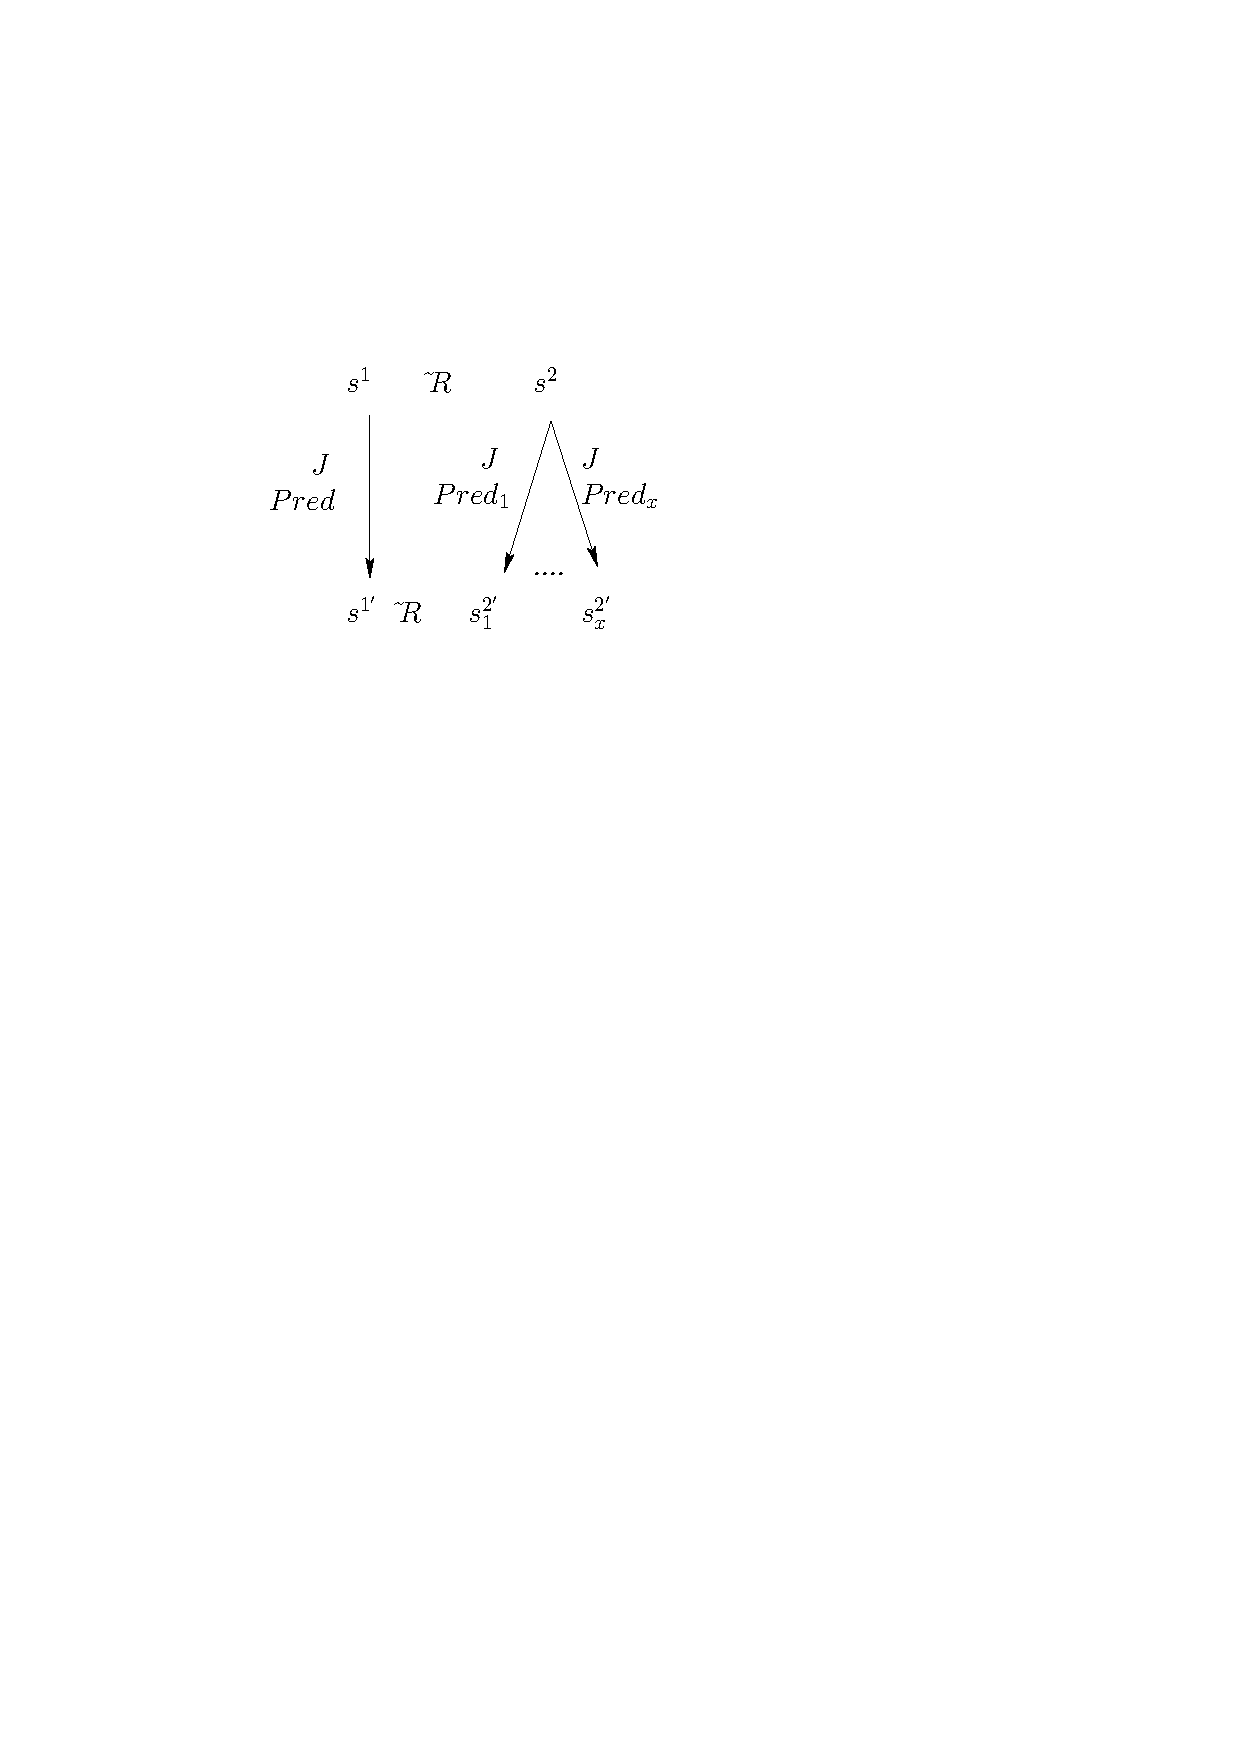
\includegraphics[width=\linewidth]{XFIG/Bisim.pdf}
\end{minipage}




 \begin{itemize}
 \item  For any open transition $OT$ in $\mathcal{T}_1$:
 \begin{mathpar}
     \openrule
         {
           \beta_j^{j\in J'},\Pred_{OT},\Post_{OT}}
         {s \OTarrow {\alpha} s'}

\end{mathpar}
 there exist   open transitions $OT_x^{x\in X} \subseteq \mathcal{T}_2$:
 \begin{mathpar}
%    \left( fresh \ \set{\alpha_i}, \set{b_j}, v_x.\ \
    \openrule
         {
           \beta_{j x}^{j\in J_{x}}, \Pred_{OT_x},\Post_{OT_x}}
         {t \OTarrow {\alpha_x} t_x}
%         \right)
\end{mathpar}
 such that  $\forall x.\, J'=J_{x}$ and there exists $\Pred_{s',t_x}$ such that $(s',t_x|\Pred_{s',t_x})\in 
 \mathcal{R}$
 and  \\
 $\Pred_{s,t} \land \Pred_{OT}\implies$\\
%\hspace{1cm}
 $\displaystyle{\bigvee_{x\in X}
   \left( \forall j. \beta_j=\beta_{jx}  \land \Pred_{OT_x}
     \land \alpha\!=\!\alpha_x \land  
     \Pred_{s',t_x}\subst{\Post_{OT}\uplus\Post_{OT_x}}\right)}$

     
 \item  and symmetrically any open transition from $t$ in $\mathcal{T}_2$ can be 
      covered by a set of transitions from $s$ in $\mathcal{T}_1$.
 \end{itemize}


 \end{definition}
Classically, $\Pred_{s',t_x}\subst{\Post_{OT}\uplus\Post_{OT_x}}$
applies in parallel the  
substitutions $\Post_{OT}$ and $\Post_{OT_x}$ (parallelism is crucial
inside each $\Post$ set but not between  $\Post_{OT}$ and
$\Post_{OT_x}$ that are independent), applying the assignments of the involved rules.
We can prove that such a bisimulation is an equivalence relation.




\begin{theorem}[FH-Bisimulation is an equivalence]\label{thm-equiv} Suppose $\mathcal{R}$ 
is an FH-bisimualtion. Then $\mathcal{R}$ is an equivalence, that is, $\mathcal{R}$ is 
reflexive, symmetric and transitive.
\end{theorem}

The proof of this theorem can be found in Annex~\ref{thm-equiv-proof}. The
only non-trivial part of the proof is the proof of transitivity. It
relies on the following elements. First,  the transitive composition
of two relations with predicate is defined; this is not exactly
standard as it requires to define the right predicate for the
transitive composition and producing a single predicate to relate any
two states. Then the fact that one open transition is simulated by a
family of open transitions leads to a doubly indexed family of
simulating open transition; this needs particular care, also because
of the use of renaming (\Post) when proving that the predicates
satisfy the definition (property on $\Pred_{s,t} \land \Pred_{OT}$ in
the definition).  


\medskip



\subsubsection*{Finite versus infinite open automata, and decidability:} 
As mentioned in Definition \pageref{def:open-automaton}, we adopt here a semantic view on open automata. More precisely, in \cite{hou:hal-02406098}, we formerly define
\emph{semantic open automata} (infinite as in Definition \ref{def:open-automaton}),
and \emph{structural open automata} (finite) that can be generated as
the semantics of pNets (see Definition \ref{def:operationalSemantics}), and used in the implementation. Then we define
an alternative version of our bisimulation, called
structural-FH-Bisimulation, based on structural open automata, and
prove that the \emph{semantic} and \emph{structural} FH-Bisimulations coincide.
In the sequel, all mentions of finite automata, and algorithms for
bisimulations, implicitly refer to their \emph{structural} versions.

If we assume that everything is finite (states and transitions in the
open automata, and the predicates in $\mathcal{R}$), then it is easy to
prove that it is decidable whether a relation is a 
FH-bisimulation, provided the logic of the predicates is
decidable (proof can be found in \cite{henrio:Forte2016}). Formally:

\begin{theorem}[Decidability of FH-bisimulation]
Let $A_1$ and $A_2$ be finite open automata
and $\mathcal{R}$ a relation over their states $\mathcal{S}_1$ and
$\mathcal{S}_2$ constrained by a finite set of predicates. Assume that
the predicates inclusion is decidable over  
the action algebra $\AlgA$. Then it is decidable whether the relation 
$\mathcal{R}$ is a FH-bisimulation.
  
\end{theorem}





\section{Weak bisimulation}\label{sec:weak}

Weak symbolic bisimulation was introduced to relate transition systems
that have indistinguishable behaviour, with respect to some definition
of \emph{internal actions} that are considered local to some
subsystem, and consequently cannot be observed, nor used for
synchronisation with their context.
The notion of non-observable actions varies in different contexts,
e.g. $tau$ in CCS, and $i$ in Lotos, we could define classically a set of
\emph{internal/non-observable actions} depending on a specific action
algebra. In this paper, to simplify the notations, we will simply use $\tau$ as the single non-observable action; the generalisation of our results to a set of non-observable actions is trivial. 
Naturally, a non-observable action cannot be synchronised with
actions of other systems in its environment. 
We show here that under such assumption of non-observability of $\tau$ actions, see Definition~\ref{def:Non-ObsTau}, we can define a weak bisimulation relation that is compositional, in the sense of open pNet composition. In this section we will first define a notion of weak open transition similar to open transition. In fact a weak open transition is made of several open transitions labelled as non-observable transitions, plus potentially one observable open transition. This allows us to define weak open automata, and a weak bisimulation relation based on these weak open automata. Finally, we apply this weak bisimulation to open pNets, obtain a weak bisimilarity relationship for open pNets, and prove that this relation has compositional properties.

%% \TODO{we should understand if it make sense to distinguish invisible
%%   from synchronised actions: in the Forte paper we wrote ``using  as 
%% \emph{invisible actions} a subset of the
%% \emph{synchronised actions} defined in Section~\ref{section:pnets}''}.

%% Proving bisimulation properties on our hierarchical broadcast example
%% would take too much space for this paper. Moreover, interesting
%% properties of the HB example would rather be adequate for weak
%% bisimulation, and its large state-space would require some
%% tool-assistance, both for the generation of the open-automata and for
%% their comparison.

\subsection{Preliminary definitions and notations}


We first specify in terms of open transition, what it means for an action to be non-observable. Namely, we constraint ourselves to system where the emission of a $\tau$ action by a sub-pNet cannot be observed by the surrounding pNets. In other words, a pNet cannot change its state, or emit a specific observable action when one of its holes emits a $\tau$ action.

More precisely, we state that $\tau$ is not observable if the automaton always allows any $\tau$ transition from holes, and additionally the global transition resulting from a $\tau$ action of a hole is a $\tau$ transition not changing the pNet's state.
We define $\Id(V)$ as the identity function on the set of variables $V$.
\begin{definition}[Non-observability of $\tau$ actions for open automata]\label{def:Non-ObsTau}
An open automaton $A = \mylangle J,\mathcal{S},s_0,V,\mathcal{T}\myrangle$ \emph{cannot observe $\tau$ actions} if and only if for all $j$ in $J$ and $s$ in $\mathcal{S}$ we have:
\begin{enumerate}
\item
\[ \openrule
         {
           (j\mapsto\tau),\True,\Id(V)}
         {s \OTarrow {\tau} s}
         \in \mathcal{T}
\]
and 
\item for all $\beta_j$, $J$,  $\alpha$,  $s$, $s'$, $\Pred$, $\Post$  such that
\[ \openrule
         {
           \beta_j^{j\in J},\Pred,\Post}
         {s \OTarrow {\alpha} s'}
         \in \mathcal{T} \] If there exists $j$ such that $\beta_j=\tau$ then we have: \[ \alpha=\tau\land s=s'\land \Pred=\True\land\Post=\Id(V) \land J=\{j\}
\]
\end{enumerate}
\end{definition}
The first statement of the definition states that the open automaton must allow a hole to do a silent action at any time, and must not observe it, i.e. cannot change its internal state because a hole did a $\tau$ transition. The second statement ensures that there cannot be in the open automaton other transitions that would be able to observe a $\tau$ action from a hole. The condition $J=\{j\}$ is a bit restrictive, it could safely be replaced by $\forall j\in J.\, \beta_j=\tau$, allowing the other holes to perform $\tau$ transitions too (because these $\tau$ actions cannot be observed).


By definition, one weak open transition contains  several open transitions, where  each open transition can require an observable action from a given hole, the same hole might have to emit several observable actions for a single weak open transition to occur. 
Consequently, for a weak open transition to trigger, a sequence of actions from a given hole may be required.

Thus, we let $\gamma$ range over sequences of action terms and use $\dotcup$ as the concatenation operator that appends sequences of action terms: given two sequences of action terms  $\gamma\dotcup\gamma '$ concatenates the two sequences. The operation is lifted to indexed sets of sequences:   at each index $i$, $\set {\gamma_1}\dotcup \set {\gamma_2}$ concatenates the sequences of actions at index $i$ of $\set{\gamma_1}$ and the one at index $i$ of $\set {\gamma_2}$\footnote{One of the two sequences is empty when $i\not \in \dom(\set{\gamma_1})$ or $i\not \in \dom(\set{\gamma_2})$ .}. $[a]$ denotes a sequence with a single element.

As required actions are now sequences of observable actions, we need an operator to build them from set of actions that occur in open transitions, i.e. an operator that takes a set of actions performed by one hole and produces a sequence of observable actions.

Thus we define $\vis{\set\beta}$ as the mapping $\set\beta$  with only observable actions of the holes in $I$, but where each element is either empty or a list of length 1:
 \[\vis{\beta_i^{i\in I}} = [\beta_i]^{i\in I'}\text{ where }I'=\left\{i| i\in I \land \beta_i\neq \tau\right\}\]

As an example the $\vis{\set\beta}$ built from the transition $OT_1$ in Example~\ref{OT:SimpleProt}, page \pageref{OT:SimpleProt} is $\texttt{P}\mapsto [\texttt{p-send(m)}]$. Remark that in our simple example no $\tau$ transition involves any visible action from a hole, so we have no $\beta$ sequences of length longer than 1 in the weak automaton.
%\TODO{en fait c'est faux ! les boucles SS\_1, SS\_2, WS\_1, WS\_2 sont aussi valides avec p\_a ou q\_b = tau, donc on peut avoir des sequences de longueur arbitraire d'actions de P et de Q}

\subsection{Weak open transition definition}

Because of the non-observability property (Definition~\ref{def:Non-ObsTau}), it is possible to add any number of $\tau$ transitions of the holes before or after any open transition freely. This property justifies the fact that we can abstract away $\tau$ transitions from holes in the definition of a weak open transition.



%
%Classically, we start by defining a derived transition relation based
%on sequences of invisible actions.

\def\InvAct{\mathcal{Inv}}
%
%\RAB{We let $\gamma$ range over words (of action terms) and use $\dotcup$ as the union that appends words.}

\begin{definition}[Weak open transition (WOT)]\label{def:weakOT}
A weak open transition over a
	set $J$ of holes with sorts $\Sort_j^{j\in J}$ and a set of states $\mathcal{S}$ is 
	a structure of the form:	
\begin{mathpar}
 \openrule
         {
           \gamma_j^{j\in J'},\Pred,\Post}
         {s \OTWeakarrow {\alpha} s'}
 \end{mathpar}
	Where $J'\subseteq J$, $s, s'\in\mathcal{S}$ and $\gamma_j$
        is a list of transitions of the hole $j$, with each element of the list in $\Sort_j$. $\alpha$ is an action 
        label denoting the resulting action
        of this open transition. \Pred\ and \Post\ are defined similarly to Definition~\ref{def:OT}. We use $\WT$ to range over sets of weak open transitions.

A weak open automaton $\mylangle J,\mathcal{S},s_0,V,\WT\myrangle$ is similar to an open automaton  except that $\WT$ is a set of weak open transitions over $J$ and $\mathcal{S}$.
\end{definition}

A weak open transition labelled $\alpha$ can be seen as a sequence of open transitions that are all labelled $\tau$ except one that is labelled $\alpha$; however conditions on predicates, effects, and states must be verified for this sequence to be fired.


We are now able to build a weak open automaton from an open automaton. This is done in a way that resembles the process of $\tau$ saturation: we add  $\tau$ open transitions before or after another (observable or not) open transition.
\begin{definition}[Building a weak open automaton]\label{def:buildweakOT}
  Let $A = \mylangle J,\mathcal{S},s_0,V,\mathcal{T}\myrangle$ be an open automaton. 
The weak open automaton \emph{derived} from $A$ is an open automaton  $\mylangle J,\mathcal{S},s_0,V,\WT\myrangle$ where $\WT$ is derived from $\mathcal{T}$ by saturation, applying the following rules:
%\noindent{\bf Invisible $\tau$ transitions:}
\begin{mathpar}
 \openrule
         {
           \emptyset,\symb{True},\Id(V)}
         {s \OTWeakarrow {\tau} s} \in \WT  \qquad \WTUn
 \end{mathpar}
and
\begin{mathpar}
\inferrule{
 \openrule
         {
           \set{\beta},\Pred,\Post}
         {s \OTarrow {\alpha} s'} \in \mathcal{T}
} 
{ \openrule
         {
           \vis{\set{\beta}}\!,\Pred,\Post
				 } {s \OTWeakarrow {\alpha} s'} \in \WT
}\qquad \WTDeux
%\inferrule{
% \openrule
%         {
%           \set{\beta},\Pred,\Post}
%         {s \OTarrow {\tau} s'} \in \mathcal{T}
%\\
% \openrule
%         {
%           \set{\gamma},\Pred\,',({x_k\gets e_k})^{k\in K}   }
%         {s' \OTWeakarrow {\tau} s''} \in \WT
%}
%{ \openrule
%         {
%           \vis{\set{\beta}}\dotcup\set{\gamma},\Pred\land\Pred\,'\subst{\Post\,},
%				({x_k\gets (e_k\subst{\Post\,})})^{k\in K} } 
%         {s \OTWeakarrow {\tau} s''} \in \WT
%}
 \end{mathpar}
 and
%\noindent{\bf Other transitions:}
\begin{mathpar}
\inferrule {\openrule
         {
           \set{\gamma_1},\Pred_1,\Post_1   }
         {s \OTWeakarrow {\tau} s_1} \in \WT
\qquad
\openrule
         {
           \set{\gamma_2},\Pred_2,\Post_2  }
         {s_1 \OTWeakarrow {\alpha} s_2} \in \WT
\qquad
\openrule
         {
           \set{\gamma_3},\Pred_3,\Post_3  }
         {s_2 \OTWeakarrow {\tau} s'} \in\WT
\\
\Pred=\Pred_1\land\Pred_2\subst{\Post_1}\land \Pred_3\subst{\Post_2\shortotimes\Post_1}
\\
\set{\gamma}=\set{\gamma_1}\dotcup \set{\gamma_2}\subst{\Post_1}\dotcup\set{\gamma_3}\subst{\Post_2\shortotimes \Post_1}\\
\alpha'=\alpha\subst{\Post_1}
}
{
\openrule
         {\set{\gamma}
           ,
		\Pred,
				\Post_3\shortotimes\Post_2\shortotimes\Post_1} 
         {s \OTWeakarrow {\alpha'} s'} \in\WT
} \WTTrois
\end{mathpar}
 
\end{definition}
Rule $\WTUn$ states that it is always possible to do a non-observable transition, where the state is unchanged and the holes perform no action. Rule~$\WTDeux$ states that each open transition can be considered as a weak open transition. The last rule is the most interesting:  Rule~$\WTTrois$ allows any number of $\tau$ transitions before or after any weak open transition. This rules carefully composes predicates, effects, and actions of the holes, indeed in the rule, predicate $\Pred_2$ manipulates variables of $s_1$ that result from the first weak open transition. Their values thus depend on the initial state but also on the effect (as a substitution $\Post_1$) of the first weak open transition. In the same manner, $\Pred_3$ must be applied the joint substitution $\Post_2\shortotimes\Post_1$. Similarly, effects on variables must be applied to obtain the global effect of the composed weak open transition, it must also be applied to observable actions of the holes, and to the global action of the weak open transition.



\subsection{Composition properties: composition of weak open transitions}
We now have two different semantics for open pNets: a strong semantics, defined  as an open automaton, and as a weak semantics, defined as a weak open automaton. Like the open automaton, the weak open automaton features valuable composition properties. We can exhibit  a composition property and a decomposition property that relate open pNet composition with their semantics, defined as weak open automata. These are however technically more complex than the ones for open automata because each hole performs a set of actions, and thus a composed transition is the composition of one transition of the top-level pNet and a sequence of transitions of the sub-pNet that fills its hole. They can be found as Lemmas~\ref{lem-decomposeWOT}, Lemma~\ref{lem-Weakcompose1}, and Lemma~\ref{lem-Weakcompose} in Appendix~\ref{sec:app-composition}.



\subsection{Weak FH-bisimulation}
For defining a bisimulation relation between weak open automata, two options are possible. Either we define a simulation similar to the strong simulation but based on open automata, this would look like the FH-simulation but would need to be adapted to weak open transitions. Or we define directly and classically a weak FH-simulation as a relation between two open automata, relating the open transition of the first one with the transition of the weak open automaton derived from the second one. 

The definition below specifies how a set of weak open transitions can simulate an open transition, and under which condition; this is used to relate, by weak FH-bisimulation, two open automata by reasoning on the weak open automata that can be derived from the strong ones.
This is defined formally as follows.

\begin{definition}[Weak FH-bisimulation]\label{def-Weak-bisim} ~\\
\noindent
Let $A_1 = \mylangle J,\mathcal{S}_1, s_0,V_1,
    \mathcal{T}_1\myrangle$ and $A_2 = \mylangle J,\mathcal{S}_2,t_0, V_2, \mathcal{T}_2\myrangle$ be open automata with disjoint sets of variables.
Let $\mylangle J,\mathcal{S}_1, s_0,V_1,
    \WT_1\myrangle$ and $\mylangle J,\mathcal{S}_2,t_0, V_2, \WT_2\myrangle$ be the
weak open automata derived from $A_1$ and $A_2$ respectively.
Let $\mathcal{R}$ a relation over
$\mathcal{S}_1$ and $\mathcal{S}_2$, as in Definition~\ref{def-FH-bisim}.

Then 
   $\mathcal{R}$ is a weak FH-bisimulation iff for any  states
$s\in\mathcal{S}_1$ and
$t\in\mathcal{S}_2$ such that $(s,t|\Pred)\in\mathcal{R}$, we 
   have the following:



 \begin{itemize}
 \item  For any open transition $OT$ in $\mathcal{T}_1$:
 \begin{mathpar}
     \openrule
         {
           \beta_j^{j\in J'},\Pred_{OT},\Post_{OT}}
         {s \OTarrow {\alpha} s'}

\end{mathpar}
 there exist weak open transitions $\symb{WOT}_x^{\;x\in X} \subseteq \WT_2$:
 \begin{mathpar}
    \openrule
         {
           \gamma_{j x}^{j\in J_{x}}, \Pred_{OT_x},\Post_{OT_x}}
         {t \OTWeakarrow {\alpha_x} t_x}
\end{mathpar}
 such that  $\forall x.\, \{j\in J'|\beta_j\neq\tau\}=J_{x}, (s',t_x|\Pred_{s',t_x})\in \mathcal{R}$; 
 and  \\
 $\Pred \land \Pred_{OT}\\
\hspace{1cm} \implies\!\!\! \displaystyle{\bigvee_{x\in X}\!
   \left( \forall j\in J_x. \vis{\beta_j}\!=\!\gamma_{jx}\! \land\! \Pred_{OT_x}
     \!\land\! \alpha\!=\!\alpha_x\! \land\!  
     \Pred_{s',t_x}\subst{\Post_{OT}\uplus\Post_{OT_x}}\right)}$
    
 \item  and symmetrically any open transition from $t$ in $\mathcal{T}_2$ can be 
      covered by a set of weak transitions from $s$ in $\WT_1$.
 \end{itemize}

Two pNets are weak FH-bisimilar if there exists a relation between their associated 
automata that is a Weak FH-bisimulation and their initial states are in the relation, i.e. 
the predicate associated to the relation between the initial states is \True.
 \end{definition}

Compared to strong bisimulation, except the obvious use of weak open transitions to simulate an open transition, the condition on predicate is slightly changed concerning actions of the holes. Indeed only the visible actions of the holes must be compared and they form a list of actions, but of length at most one.




Our first important result is that Weak FH-bisimilarity is an equivalence in the same way as strong FH-bisimilarity:


\begin{theorem}[Weak FH-Bisimulation is an equivalence]\label{thm-weak-equiv} Suppose $\mathcal{R}$ 
is a weak FH-bisimulation. Then $\mathcal{R}$ is an equivalence, that is, $\mathcal{R}$ is 
reflexive, symmetric and transitive.
\end{theorem}
The proof  is detailed in Appendix \ref{app-WFH-equiv}, it follows a similar pattern as the proof that strong FH-bisimulation is an equivalence, but technical details are different, and in practice we rely on a variant of the definition of weak FH-bisimilarity; this equivalent version simulates a \emph{weak} open transition with a set of weak open transition. The careful use of the best definition of weak FH-bisimilarity makes the proof similar to the strong FH-bisimulation case.

\subsubsection*{Proving bisimulation in practice}

In practice, we are dealing with finite representations of the (infinite) open automata. In \cite{hou:hal-02406098}, we defined a slightly modified definition of the ``coverage'' proof obligation, in the case of strong FH-Bisimulation. This modification is required to manage in a finite way all possible instantiations of an OT. In the case of weak FH-Bisimulation, the proof obligation from Definition \ref{def-Weak-bisim} becomes:
      \begin{multline*}
\forall fv_{OT}.\, \Big\{ \Pred \land \Pred_{OT} \implies\\
 \bigvee_{x\in X}\!
  \left[\exists fv_{OT_x}.
    \left( \forall j\in J_x. \vis{\beta_j}\!=\!\gamma_{jx}\! \land\! \Pred_{OT_x}
     \!\land\! \alpha\!=\!\alpha_x\! \land\!  
     \Pred_{s',t_x}\subst{\Post_{OT}\uplus\Post_{OT_x}}\right)\right]\Big\}
\end{multline*}

In which $fv_{OT}$ denotes the set of free variables of all expressions in $OT$.





\bibliographystyle{lncs/splncs}

% \bibliography{oasis,biblio}
\bibliography{biblio}

\newpage
\appendix    




\section{Parameterised Networks (pNets)}
\label{section:pnets}

pNets are tree-like structures, where the leaves are either \emph{parameterised labelled transition systems (pLTSs)}, expressing the
behaviour of basic processes, or \emph{holes}, used as placeholders
for unknown processes. 
%, of which we only specify the set of possible
%actions, this set is named the \emph{sort}.
Nodes of the tree (pNet nodes) are synchronising artefacts, using a
set of \emph{synchronisation vectors} that express the possible
synchronisation between the parameterised actions of a subset of the sub-trees.

%\LUDO{introduce magic op}
%$\CreateISet{a}{i}$ creates a single entry indexed set $(i\mapsto a)$ \emph{but only if 
%$a$ is not already an indexed set.}


A pLTS is a labelled transition system with variables; variables can be
used inside states, actions, guards, and
assignments. 
%Similarly, to simplify the management of variables and without loss of expressivity, we 
%suppose that transitions looping to the same state does not do assignments.
Note that we make no assumption on finiteness of the set of states nor
on finite branching of the transition relation. Compared to our previous works~\cite{henrio:Forte2016,AmeurBoulifa2017} we extend the expressiveness of the model by making variables global.


\begin{definition}[pLTS]
\label{pLTS}
A pLTS is a tuple
$\pLTS\triangleq\mylangle S,s_0, V, \to\myrangle$ where:
\begin{itemize}
\item[$\bullet$]
$S$ is a set of states.
\item[$\bullet$]
$s_0 \in S$ is the initial state.
%\item[$\bullet$]
 %Variables in
%$\iv(\alpha)$ are assigned by the action, other variables can be assigned
%by the additional assignments.
\item[$\bullet$] $V$ is a set of global variables for the pLTS,
\item[$\bullet$] $\to \subseteq S \times L \times S$ is the transition relation and 
$L$ is the set of labels of the form:\\
$\langle \alpha,~e_b,~(x_j\!:= {e}_j)^{j\in J}\rangle$,
where $\alpha \in\AlgA$ is a parameterised action, $e_b \in
\AlgB$ is a guard, and the variables $x_j$ 
are assigned the expressions $e_j\in \AlgE$.
If 
$s \xrightarrow{\langle \alpha,~e_b,~(x_j\!:= {e}_j)^{j\in
		J}\rangle} s'\in \to $ then 
% REMOVED BECAUSE USELESS: $\iv(\alpha)\!\subseteq\! \vars(s')$, 
		$\vars(\alpha)\backslash \iv(\alpha)\!\subseteq\! V$, 
		$\vars(e_b)\!\subseteq\! \vars(s)\cup\vars(\alpha)$, and
		$\forall j\!\in\! J .\,\left(\vars(e_j)\!\subseteq\! V\cup\iv(\alpha)\land 
		x_j\!\in V \right)$. %,  and $s= s'\Rightarrow J=\emptyset$.

%\LUDO{I suggest to add: $\{x_j|j\in J\} = \vars(s')$ or $\{x_j|j\in J\} \cup \iv(\alpha)= \vars(s')$} 
\end{itemize}
\end{definition}

The semantics of the assignments is that a set of assignments between two states is performed in parallel so that their order do not matter and they all use the values of variables before the transition (or the values received as action parameters).


Now we define
pNet nodes as constructors for hierarchical behavioural structures.
A pNet has a set of sub-pNets that can be either pNets or pLTSs, and a
set of holes, playing the role of process parameters. A pNet is thus a composition operator that can receive processes as parameters; it expresses how the actions of the sub-processes synchronise.

Each sub-pNet exposes
a set of actions, called \emph{internal actions}. The synchronisation between global actions exposed by the pNet and
internal actions of its sub-pNets is given by  \emph{synchronisation vectors}: a
synchronisation vector synchronises one or several internal actions, and
exposes a single resulting global action.


We now define the structure of pNets, the following definition relies on the definition 
of holes, leaves and sorts formalised below in Definition~\ref{def-sortholeleave}. Informally, holes are process parameters, leaves provide the set of pLTSs at the leaves of the hierarchical structure of a pNet, and sorts give the signature of a pNet, i.e. the actions it exposes.

\begin{definition}[pNets]\label{def-pnets}
A pNet $\pNet$ is a hierarchical structure where leaves are pLTSs and holes:\\
$\pNet\triangleq \pLTS~|~\mylangle \pNet_i^{i\in I}, \Sort_j^{j\in J}, \symb{SV}_k^{k\in 
K}\myrangle$
where
\begin{itemize}
\item[$\bullet$] $\pNet_i^{i\in I}$ is the family of sub-pNets indexed over $I$. $vars(P_i)$ and $vars(P_j)$ must be disjoint for $i\neq j$.
%  $\pNet_i^{i\in I}$ is a family of sub-pNets where $I\in\I_\P$ is the set over which sub-pNets are indexed.

\item[$\bullet$] $J$ is a set of indexes, called \emph{holes}.
$I$ and $J$ are \emph{disjoint}: $I\!\cap\! J=\emptyset$,  $I\!\cup\! J\neq\emptyset$
\item[$\bullet$] $\Sort_j \subseteq \AlgAS$  is a set of action terms, denoting the 
\emph{sort} of
hole $j$.

\item[$\bullet$] $\symb{SV}_k^{k\in K}$ is a set of
  synchronisation vectors. $\forall k\!\in\! K.\,
  \symb{SV}_k\!=\!\SV{\alpha_{l}^{l\in I_k \uplus J_k}}{\alpha'_k}{e_k}$ where
  $\alpha'_k\in \AlgAS$, $I_k\subseteq I$, $J_k\subseteq J$,
  $\forall i\!\in\!
  I_k.\,\alpha_{i}\!\in\!\Sort(\pNet_i)$,  $\forall j\!\in\!
  J_k.\,\alpha_{j}\!\in\!\Sort_j$, and $\vars(\alpha'_k)\subseteq \bigcup_{l\in I_k\uplus 
  J_k}{\vars({\alpha_l})}$. The global action of a vector $\symb{SV}_k$ is
$\alpha'_k$. $e_k \in \AlgB$ is a guard associated to the vector such that
$\vars(e_k)\subseteq \bigcup_{l\in I_k\uplus J_k}{\vars({\alpha_l})}$.
\end{itemize}
Synchronisation vectors are identified modulo renaming of variables that appear in their 
action terms.
\end{definition}

The preceding definition relies on the auxiliary functions defined below:

\begin{definition}[Sorts, Holes, Leaves, Variables of pNets]\label{def-sortholeleave}~~

  \begin{itemize}
  \item The sort of a pNet is its signature, i.e. the set of actions in $\AlgAS$ it can
perform, where each action signature is an action 
label plus the arity of the action. In the definition of sorts, we do not need to 
distinguish
input variables and we remove the
\emph{input marker} (?) of variables.
\[
\begin{array}{l}
\Sortop(\mylangle S,s_0,V, \to\myrangle) = \{\alpha\subst{?x \gets x| 
x\in\symb{iv}(\alpha)}|s \xrightarrow{\langle \alpha,~e_b,~(x_j\!:= {e}_j)^{j\in
    J}\rangle} s'\in \to \} \\
\Sortop(\mylangle \set{\pNet}\!, %\pNet_i^{i\in I}, 
\set{\Sort},
\set{\symb{SV}\,}\myrangle)
=\{\alpha' |\, \SV{\set{\alpha}}{\alpha'}{e_b}\in\set{\symb{SV}}\,\}
\end{array}
\]

\item The set of variables of a pNet $P$, denoted $vars(P)$ is disjoint union the set of variables of  all pLTSs that compose $P$.

\item
The set of holes $\Holes(\pNet)$ of a pNet is the indexes of the holes of the pNet 
itself plus the indexes of all the holes of its sub-pNets.
It is defined inductively (we suppose those indexes 
disjoints):
  \[\begin{array}{l}
\Holes(\mylangle S,s_0,V, \to\myrangle) \!=\! \emptyset\\
\Holes(\mylangle \pNet_i^{i\in I}\!,\set{\Sort}, \set{\symb{SV}}\myrangle) 
=J\uplus{\displaystyle \bigcup_{i\in 
I}\Holes(\pNet_i)}\\
\forall i\in I.\, \Holes(\pNet_i)\cap J=\emptyset\\
\forall i_1,i_2\in I.\,i_1\neq i_2\Rightarrow  \Holes(\pNet_{i_1})\cap\Holes(\pNet_{i_2})=\emptyset
\end{array}\]
\item
The set of leaves of a pNet is the set of all pLTSs occurring in the structure, as an 
indexed family of the form $\Leaves(\pNet)= \mylangle \pNet_i \myrangle^{i \in L}$.
\[\begin{array}{l}
\Leaves(\mylangle S,s_0,V, \to\myrangle) \!=\!\emptyset\\%\{\mylangle S,s_0, \to\myrangle\}\\
\Leaves(\mylangle \pNet_i^{i\in I}\!,%Sort_j^{j\in J}
\set{\Sort}\!, \set{\symb{SV}\,}\myrangle) = {\displaystyle \biguplus_{i\in 
I}\Leaves(\pNet_i)\uplus\{i\mapsto \pNet_i|\pNet_i \text{ is a }\pLTS\}}
\end{array}\]
\end{itemize}

A pNet $Q$ is \emph{closed} if it has no hole: $\Holes(Q)=\emptyset$; else it
is said to be \emph{open}.
\end{definition}
  
The informal semantics of pNets is as follows. pLTSs behave more or less like  classical automata with conditional branching and variables. The actions on the \pLTS s can send or receive values, potentially modifying the value of variables. 
pNets are synchronisation entities: a pNet composes several sub-pNets and  synchronisation vectors define how the sub-pNets interact, where a sub-pNet is either a pNet or a pLTS. Synchronisation between sub-pNets is defined by synchronisation vectors that express how an action of a sub-pNet can be synchronised with actions of other sub-pNet, and how the resulting synchronised action is visible to the outside of the pNet. Synchronisation vectors can also express the exportation of an action of a sub-pNet to the next level, or to hide an interaction and make it non-observable. Finally, a pNet can leave sub-pNets undefined and instead declare holes with a well-defined signature. Holes can then be filled with a sub-pNet. This is defined as follows.



\begin{definition}[pNet composition]
	An open pNet: $\pNet = \mylangle \pNet_i^{i\in I}, \Sort_j^{j\in J}, 
	\set{\symb{SV}}\,\myrangle$
 can be (partially) filled by providing  a pNet $\pNetQ$ of the
	right sort to fill one of  its holes.	
	Suppose $j_0\in J$:
	%% \[\mylangle \pNet_i^{i\in I},S_j^{j\in J}, \symb{SV}_k^{k\in
	%%   K}\myrangle\left[(\pNet'_i)^{i\in L}\right]= \mylangle \pNet_i^{i\in
	%%   I}\left[(\pNet'_i)^{i\in L}\right]\uplus(\pNet'_i)^{i\in J\cap L},S_j^{j\in 
	%%J\setminus L},
	%% \symb{SV}_k^{k\in K}\myrangle
	%% \]
	\[\pNet\left[\pNetQ\right]_{j_0}= \mylangle 
	\pNet_i^{i\in I}\uplus\{j_0\mapsto \pNetQ\},\Sort_j^{j\in J\setminus \{j_0\}},
	\set{\symb{SV}}\,\myrangle
	\]
\end{definition}

pNets are composition entities equipped with a rich synchronisation mechanism: synchronisation vectors allow the expression of synchronisation between any number of entities and at the same time the passing of data between processes. Their strongest feature is that the data emitted by processes can be used can be used inside the synchronisation vector to do addressing: it is easy to synchronise a process indexed by $n$ with the action $a(v,n)$ of another process. This is very convenient to model systems and encode futures or message routing. pNets have been used to model GCM distributed component systems, illustrating the expressiveness of the model~\cite{AmeurBoulifa2017}. These works show that pNets are convenient to express the behaviour of the system in a compositional way, which is crucial for the definition of the semantics, especially when dealing with a hierarchical component system like GCM. Unfortunately, the semantics of pNets and the existing tools at this point were only able to deal with a closed system completely instantiated: pNets could be used as composition operator in the definition of the semantics, which was sufficient to perform finite-state model checking on a closed system, but there was no theory for the use of pNets as operators and no tool for proving properties on open system. The semantics of closed pNets~\cite{AmeurBoulifa2017}, defined as an instantiation of labelled transition systems, is not necessary to understand this article but can be useful to  understand the semantics of pNets in a simpler and more operational setting. The theory of pNets as operators able to fully take into account open systems is given in the following sections.




\section{Semantics of Open pNets}
\label{section:op-semantics}

This section defines the semantics of an open pNet as a translation into an open automaton. 
In this translation, the states of the open automata are obtained from
the states of the pLTSs at the leaves of the composition. The
predicates on the transitions are obtained both from the predicates on
the pLTSs transitions and from the synchronisation vectors involved in
the transition. 

The definition of bisimulation for open automata allows us to derive a
bisimulation theory for open pNets. As pNets are composition
structures, it then makes sense to prove composition lemmas: we prove
that the composition of strongly bisimilar pNets are themselves
bisimilar. 

\subsection{Deriving an open automaton from an open pNet}
To derive an open automaton from a pNet, we need to describe the set of states of the automaton, and then we will detail the construction rule for transitions of the automaton, this will rely on the derivation of predicate unifying synchronisation vectors and the actions of the pNets involved in a given synchronisation.

%Then the semantics of a pNet is characterized by a set of {\em open
%transitions}, where the hypotheses on process parameters are
%replaced by 1) transitions of the pLTSs at the leaves, and 2) formal
%hypotheses on the transitions of the holes. A {\em predicate} is used
%to relate the parameters and names appearing in the actions of the
%leaves and the holes involved in the rules, but also appearing in  the resulting action.

We first define states of open pNets as tuples of states. We denote them
 as $\triangleleft\ldots\triangleright$ for distinguishing tuple 
states from other tuples.
\begin{definition}[States of open pNets]\label{def-states}
  A state of an open pNet is a tuple (not necessarily finite) of the
  states of its leaves.

  For any pNet \pNet, let $\Leaves(\pNet) = \mylangle S_i,{s_i}_0,V, \to_i\myrangle^{i \in L}$ be 
  the set of pLTS at its leaves,
  then $States(\pNet) = \{\triangleleft s_i^{i\in L}
  \triangleright| \forall i\in L. s_i \in S_i\}$.
A pLTS being its own single leave:\\
  $States(\mylangle S,s_0,V, \to\myrangle) = \{\triangleleft s \triangleright| s \in S \}$.  
%This could be encoded as a mapping from variables of the pNet to expressions, of the form: $\sigma=\{x_i\to e_i\}^{i\in I},\,(x_i\in vars(S))$.
%\LUDO{j ai ajoute les variables mais c est pas tres beau}

The initial state is defined as:
$InitState(\pNet) = \triangleleft {{s_i}_0}^{i\in L}  \triangleright$.
\end{definition}
To be precise, the state of each pLTS is entirely characterised by both the state of the automaton, and the value of its variables $V$. Consequently, the complete characterization of the state of a pNet should take into account the value of its variables $vars(P)$.


%% \begin{example} \emph{State of a pNet}
%%   The states of pNet \texttt{EnableCompL} are:
%%   $\triangleleft 00 \triangleright, \triangleleft 10 \triangleright, \triangleleft 11 \triangleright$
%% \end{example}

\subsubsection*{Predicates} 
%Let
%$\mylangle\set{\pNet},\set{\Sort},\set{\symb{SV}}\myrangle$
%be a pNet. 
Consider a synchronisation vector $\SV{{(\alpha'_i)}^{i\in I}, {(\beta'_j)}^{j\in J}} 
{\alpha'} 
{e_b}$. We 
define a
predicate $\Predsv$ relating
the actions of the involved sub-pNets and the resulting actions. This predicate verifies:
\[\begin{array}{l}\Predsv \Big(\SV{{(\alpha'_i)}^{i\in I}, {(\beta'_j)}^{j\in J}} 
{\alpha'} 
{e_b}, \alpha_i^{i\in I}, \beta_j^{j\in J}, \alpha\Big)\Leftrightarrow \\~\qquad\qquad%\bigg(
%
%\exists {(\alpha'_i)}^{i\in I},
%{(\beta'_j)}^{j\in J},v'.\, SV=
%\\~~\land
\forall i\in I.\, \alpha_i=\alpha'_i\land \forall j \in J.\, \beta_j=\beta'_j \land 
\alpha=\alpha' 
\land e_b
\end{array} 
%\bigg)
\]

Somehow, this predicate entails a verification of satisfiability in the sense that if the 
predicate $\Predsv$ is not satisfiable, then the transition associated with the 
synchronisation will not occur in the considered state, or will occur with a \False\ precondition which is equivalent.
If the action families do not match or if there is no valuation of
variables such that the above formula can be ensured then the predicate is undefined.

The definition of this predicate is not constructive but it is easy to build the predicate constructively by brute-force unification of the sub-pNets actions with the corresponding vector actions, possibly followed by a simplification step.


\section{pNet Composition Properties: composition of open transitions}
The semantics of open pNets allows us to prove two crucial properties relating pNet composition with pNet semantics: open transition of a composed pNet can be decomposed into open transitions of its composing sub-pNets, and conversely, from the open transitions of sub-pNets,  an open transition of the composed pNet can be built.

We start with decomposition: from one open transition of $P[Q]_{j_0}$, we exhibit 
corresponding behaviours of $P$ and $Q$, and determine the relation between their 
predicates:
\begin{lemma}[Open transition decomposition\label{lem-decompose}] Consider two pNets $P$ and $Q$ that are not pLTSs\footnote{A similar lemma can be proven for a pLTS $Q$}.
	Let $\Leaves(Q)=p_l^{l\in L_Q}$; suppose:
	\[ P[Q]_{j_0}  
		\models
		{\openrule
			{
				\beta_j^{j\in J}, \Pred,  
				\Post}
			{\ostate{s_i^{i\in L}} \OTarrow {\alpha}
				\ostate{s_i'^{\, i\in L}}}
		}
	\]
		with  $J\cap\Holes(Q)\neq\emptyset$ or $\exists i\in L_Q.\,s_i\neq s'_i$, i.e. $Q$ takes part in the reduction.
		 Then there exist $\alpha_Q$, $\Pred\,'$, $\Pred\,''$, 
		$\Post\,'$, $\Post\,''$ s.t.:\\[-2ex]
		%\[
		\begin{mathpar}
		P\models{\openrule
			{
				\beta_j^{j\in (J\setminus \Holes(Q)) \cup \{j_0\}}, 
				\Pred\,',  
				\Post\,'}
			{\ostate{s_i^{i\in L\setminus L_Q}} \OTarrow {\alpha}
				\ostate{s_i'^{\,i\in L\setminus L_Q}}}
		}%\]
	\vspace{-2.2ex}\\\text{and~~}
		%\[
		Q\models{\openrule
			{
				\beta_j^{j\in J\cap\Holes(Q)}, \Pred\,'',  
				\Post\,''}
			{\ostate{s_i^{i\in L_Q}} \OTarrow {\alpha_Q}
				\ostate{s_i'^{\,i\in L_Q}}}
		}%\]
		\end{mathpar}
		and  $\Pred \iff \Pred\,'
		\land \Pred\,''\land \alpha_Q=\beta_{j_0}$, $\Post=\Post\,'\uplus 
		\Post\,''$ where $\Post\,''$ is the restriction of $\Post$ over variables of 
		$Q$.
\end{lemma}


Lemma \ref{lem-compose} is combining an open transition of $P$ with
an open transition of $Q$, and building a corresponding transition of
$P[Q]_{j_0}$, assembling their predicates.

\begin{lemma}[Open transition composition]\label{lem-compose} 
	Suppose $j_0\in J$ and:\\[-2ex]
\begin{mathpar}
%\[
P\models{\openrule
	{
		\beta_j^{j\in J}, 
		\Pred,  
		\Post}
	{\ostate{s_i^{i\in L}} \OTarrow {\alpha}
		\ostate{s_i'^{\, i\in L}}}
}%\]
\text{~~and~~}
%\[
Q\models{\openrule
	{
		\beta_j^{j\in J_Q},
		 \Pred\,',  
		\Post\,'}
	{\ostate{s_i^{i\in L_Q}} \OTarrow {\alpha_Q}
		\ostate{s_i'^{\, i\in L_Q}}}
}%\]
\end{mathpar}
Then, we have\\[-2ex]
	\[ P[Q]_{j_0}  
	\models
	{\openrule
		{
			\beta_j^{(j\in J\setminus\{j_0\}) \uplus J_Q}, 
			\Pred\land\Pred\,'\land \alpha_Q=\beta_{j_0},  
			\Post\uplus \Post\,'}
		{\ostate{s_i^{i\in L\uplus L_Q}} \OTarrow {\alpha}
			\ostate{s_i'^{\, i\in L\uplus L_Q}}}
	}
	\]
\end{lemma}

Note that this does not mean that any two pNets can be composed and produce an open 
transition. Indeed, the predicate $\Pred\land\Pred\,'\land \alpha_Q=\beta_{j_0}$ is often not  satisfiable, in particular if the action  $\alpha_Q$ cannot be matched with $\beta_{j_0}$.
Note also that $\beta_{j_0}$ is  only used as an intermediate term inside formulas in the composed open transition: it 
does not appear neither as global action nor as an action of a hole.




We build the semantics of open pNets as an open automaton over the states  given by 
Definition~\ref{def-states}. The open transitions first
 project the global state into states of the leaves, then apply
pLTS transitions on these states, and compose them with the sort of the holes. %The pNet
%structure does not appear in the open-automaton, only the
%set of Holes and the set of Leaves.
The semantics    instantiates fresh variables using the predicate $\fresh(x)$, additionally, for an action 
$\alpha$, $\fresh(\alpha)$ means all variables in $\alpha$ are fresh.


\begin{definition}[Semantics of open pNets]
	\label{def:operationalSemantics} The semantics of a pNet $\pNet$ is an open automaton $A\!= 
	\mylangle \symb{Holes}(\pNet),\symb{States}(\pNet),\symb{InitState}(\pNet),\symb{vars}(P),\mathcal{T} \myrangle$ where $\mathcal{T}$   is the smallest set of open transitions such that $\mathcal{T}=\{OT\,|\,\pNet \models OT \}$ and	$\pNet \models OT$	is defined by the following  rules:
%	\begin{itemize}
%		\item $J$ is the set of holes: $Holes(p)= J$. 
		%  \item $\set{L}^L = Leaves(p), \set{H}^J = Holes(p)$
%		\item ${\mathcal{S}} = States(p)$ and $s_0 = InitState(p)$
%		\item $\mathcal{T}$ is the smallest set of open transitions		satisfying the rules below:
%	\end{itemize}
	
	%% \TODO{ We should be careful here: after (re) reading "Huimin
	%% 	Lin, 'Symbolic Transition Systems with Assignements', Concur'96" I
	%% 	think handling assignments is not trivial, even for comparisons of pLTSs. }


	
\begin{itemize}
\item The rule for a pLTS  checks that the guard is verified and transforms assignments into post-conditions:		
\begin{mathpar}\inferrule
		{ s \xrightarrow{\langle \alpha,~e_b,~(x_j\!:= {e}_j)^{j\in
					J}\rangle} s'\in \to  }
		{ \mylangle  S,s_0, \to \myrangle
			\models
			\openrule
			{\emptyset ,
			e_b,\left\{x_j\gets e_j\right\}^{j\in J}}
			{\ostate{s} \OTarrow{\alpha} \ostate{s'}}
		}\quad {\TrUn}
\end{mathpar}
%	Note that this note is greatly simplified by the fact that variables are local to 
%	thread; introducing global state variables or accepting loops to the same 
%	state would 
%	require to reason 
%	on the scope of 
%	each variables, and to introduce additional variables to handle the several occurence 
%	of the same pLTS variable in the predicates. Indeed the constraints on pLTS 
%	transitions 
%	ensure that the same variable never appears both on the left and on the right of the 
%	equations of a predicate.
	
\item	The second rule deals with pNet nodes: for each possible
	synchronisation vector (of index $k$) applicable to the rule subject, the premisses
	include one {\em open transition} for each sub-pNet involved, one possible
	{\em action} for each hole involved, and the predicate relating these
	with the resulting action of the vector. The sub-pNets involved are split between two 
	sets, $I_2$ for sub-pNets that are pLTSs, and $I_1$ for the others, $J$ is the set of 
	holes involved in the transition\footnote{Formally, if $SV_k \!=\! \SV{({\alpha'})_m^{m 
	\in M}}{\alpha'}{e_b}$ is a synchronisation vector  of \pNet\  then $J=M\cap 
	\Holes(\pNet)$, $I_2=M\cap \Leaves(\pNet)$,  $I_1=M\setminus J \setminus 
	I_2$}.                                                                    
\begin{mathpar}
    \mprset {vskip=.45ex}
\inferrule
    {
\Leaves(\mylangle {\pNet}_m^{m\in I}, \set{\Sort}, \symb{SV}_k^{\,k\in 
    	K}\myrangle) \!=\! \pLTS_l^{\,l\in L} \quad  	
k\!\in\! K \quad SV_k \!=\! \SV{(\alpha'_m)^{m \in I_1\uplus I_2\uplus J}}{\alpha'}{e_b} 
\\
\\     	
	\forall m\!\!\in\!\! I_1. {\pNet_m 
	\models\openrule
    	{\beta_{j}^{j\in J_m}, \Pred_m, \Post_m}
    	{\ostate{s_{i}^{i \in L_m}} \OTarrow {\alpha_m}
    		\ostate{(s_i^\prime)^{i\in L_m}}} }	
  \qquad
\forall m\!\!\in\!\! I_2.		{ \pNet_m 
    	 \models
    	\openrule
    	{\emptyset, \Pred_m, \Post_m}
    	{\ostate{s_m} \OTarrow {\alpha_m}
    		\ostate{s_m'}} }\\\\
    J' = \biguplus_{m\in I_1}\!\! J_m \uplus J	\\
    	\Pred = \bigwedge_{m\in I_1\uplus I_2}\!\! \Pred_m \land
    	\Predsv(SV_k,\alpha_m^{m\in I_1\uplus I_2},\beta_j^{j\in J},\alpha)\\ 
    	\forall i\in	L\backslash \left(\biguplus_{m\in I_1}\!\! L_m \uplus I_2\right).\,s'_i=s_i \\
    \fresh(\alpha'_m,\alpha',\beta_j^{j\in J},\alpha) 
    }
    {\mylangle {\pNet}_m^{m\in I}, \set{\Sort}, \symb{SV}_k^{\,k\in K}\myrangle
    	\models
    	{\openrule
    		{
    		\beta_j^{j\in J^\prime}, \Pred,  \biguplus_{m\in I_1\uplus I_2} 
    		\Post_m}
    		{\ostate{s_i^{i\in L}} \OTarrow {\alpha}
    			\ostate{(s_i^\prime)^{i\in L}}}
    	}
    }\quad {\TrDeux}
\end{mathpar} 
\end{itemize} 
	\medskip
%        \TODO{may be explain how $\Pred(SV,a_i^{i\in I_k},b_j^{j\in
%            J_k},v)$ is built ? You mean more than what is written on previous page????}
	%%    \TODO{I have tentatively added the sort constraint on hole actions, that was
	%%not included in the first version... I'm unsure whether this is the best place to
	%%include it, because it may change the decidability conditions on predicates}
\end{definition}
        	A key to understand this rule is that the open transitions are
	expressed in terms of the leaves and holes of the whole pNet structure,
	i.e. a flatten view of the pNet. For example, $L$ is the index set of the
	Leaves, $L_m$ the index set of the leaves of one sub-pNet indexed $m$, so all $L_m$
	are disjoint subsets of $L$. Thus the states in the open transitions,
	at each level, are tuples including states of all the
	leaves of the pNet, not only those involved in the chosen
	synchronisation vector.


Note that  the construction is symbolic, and each open-transition deduced expresses a whole family of
behaviours, for any possible value of the variables.
%

In \cite{henrio:Forte2016}, we have shown a detailed example of the construction of a complex open transition, building a deduction tree using rules \TrUn ~and \TrDeux.



We have shown in \cite{henrio:Forte2016} that an open pNet
with finite synchronisation sets, finitely many leaves and
holes, and each pLTS at leaves having a finite number of states and
(symbolic) transitions, has a finite automaton. The algorithm for building such an automaton can be found in~\cite{QBMZ-AVOCS18}.



\section{Bisimulation for open pNets -- a composable bisimulation theory}
\label{section:bisimulation-PN}
As  our symbolic operational semantics provides an open automaton, we can apply the notion of
	strong (symbolic) bisimulation on automata to open pNets:
\begin{definition}[FH-bisimulation for open pNets]\label{def:bisim-pnets}
Two pNets are FH-bisimilar if there exists a relation between their associated 
automata that is an FH-bisimulation and their initial states are in the relation (i.e. the predicate associated with the initial states is verifiable).
%\TODO{check}
\end{definition}
%\TODO{Predicate=True me pose un probleme... typiquement, on a besoin d'une ``condition initiale'', pour avoir des pNets data-oriented equivalents a leur version state-oriebted => remove the constraint}

We can now prove that pNet composition  preserves
FH-bisimulation. More precisely, one can define two preservation
properties, namely 1) when one hole of a pNet is filled by two bisimilar other (open) pNets; and 2) when the same hole in two bisimilar pNets are
filled by the same pNet, in other words, composing a pNet with two
bisimilar contexts. The general case will be obtained by
transitivity of the bisimulation relation (Theorem~\ref{thm-equiv}). 

\begin{theorem}[Congruence]\label{thm-congr-eq}
	Consider an open pNet:
	$\pNet = \mylangle \pNet_i^{i\in I}, \Sort_j^{j\in J}, 
	\set{\symb{SV}}\myrangle$.
	Let $j_0\in J$ be a hole. Let $\pNetQ$ and $\pNetQ'$ be two FH-bisimilar pNets such that\footnote{Note that $\Sortop(\pNetQ)=\Sortop(\pNetQ')$ is 
	ensured by 
	strong bisimilarity.} 
	$\Sortop(\pNetQ)=\Sortop(\pNetQ')=\Sort_{j_0}$. Then 
	$\pNet[\pNetQ]_{j_0}$ and 
	$\pNet[\pNetQ']_{j_0}$ are FH-bisimilar.
\end{theorem}
 
 
\begin{theorem}[Context equivalence]\label{thm-ctxt-eq}
	Consider two  open pNets
	$\pNet = \mylangle \pNet_i^{i\in I}, \Sort_j^{j\in J}, 
	\set{\symb{SV}}\myrangle$ and 	$\pNet' = \mylangle {\pNet'}_i^{i\in I}, 
	\Sort_j^{j\in 
	J}, 	\set{\symb{SV'}}\myrangle$ that are FH-bisimilar
	(recall they must have the same holes to be bisimilar).
	Let $j_0\in J$ be a hole, and $Q$ be a pNet such that $\Sortop(Q)=\Sort_{j_0}$. Then 
	$\pNet[Q]_{j_0}$ and 
	$\pNet'[Q]_{j_0}$ are FH-bisimilar.
\end{theorem}

Finally, the previous theorems can be composed to state a general theorem about 
composability and FH-bisimilarity.
\begin{theorem}[Composability] \label{thm-composability}
	Consider two FH-bisimilar pNets with an arbitrary number of holes, when replacing, 
	inside those two original pNets, a subset of the holes by FH-bisimilar pNets, we 
	obtain two FH-bisimilar pNets.
\end{theorem}
This theorem is quite powerful. It somehow implies that the theory of open pNets is convenient to study properties of process composition. Open pNets can indeed be used to study process operators and process algebras, as shown in~\cite{henrio:Forte2016}, or to study interaction protocols~\cite{BHHM:FACS11}.

\section{Weak bisimulation for open pNets}

Before defining a weak open automaton for the semantics of open pNets,
it is necessary to state under which condition a pNet is unable to
observe silent actions of its holes. In the setting of pNets this can
simply be expressed as a condition on the synchronisation
vectors. Precisely, the set of synchronisation vectors must contain
vectors that let silent actions go through the pNet,
i.e. synchronisation vectors where one hole does a $\tau$ transition,
and the global visible action is a $\tau$. Additionally, no other
synchronisation vector must be able to react on a silent action from a
hole, i.e. if a synchronisation vector observes a $\tau$ from a hole
it cannot synchronise it with another action nor emit an action that
is not $\tau$. This is formalised as follows:



\begin{definition}[Non-observability of silent actions for pNets]\label{def:non-obspNet}~\\
A pNet $\mylangle \pNet_i^{i\in I} , \Sort_j^{j\in J}, \set{\symb{SV}}\myrangle$
 \emph{cannot observe silent actions} if it verifies:\\ $\forall i\in I\uplus J.\, \SV{(i\mapsto \tau)}{\tau}{\True}\in \set{\symb{SV}}$ and 
\begin{equation*}
%\begin{split}
\forall \left(\SV{{(\alpha_i)}^{i\in I'}} 
{\alpha'} 
{e_b}\in \set{\symb{SV}}\right), %&
\forall i\in I'\cap J.\, \alpha_i=\tau \implies %\\
%& 
\alpha'=\tau ~\land~ %\\
%&
I'=\{i\}
%\end{split}
\end{equation*}
\end{definition}

With this definition, it is easy to check that the open automaton that gives the semantics of such an open pNet cannot observe silent actions in the sense of Definition~\ref{def:Non-ObsTau}:

\begin{property}[Non-observability of silent actions]
The  semantics of a pNet, as provided in Definition~\ref{def:operationalSemantics}, that cannot observe silent actions is an open automaton that  cannot observe silent actions.
\end{property}

%\TODO{question : we could merge prop 1 and def above, is it better?}

Under this condition, it is safe to define the weak open automaton that provides a weak semantics to a given pNet. This is simply obtained by applying Definition~\ref{def:buildweakOT} to generate a weak open automaton from the open automaton that is the strong semantics of the open pNet, as provided by Definition~\ref{def:operationalSemantics}.

\begin{definition}[Semantics of pNets as a weak open automaton]
Let $A$ be the open automaton expressing the semantics of an open pNet $\pNet$; let $\mylangle J,\mathcal{S},s_0, V, \WT\myrangle$ be the weak open automaton derived from $A$; this weak open automaton defines the weak semantics of the pNet $\pNet$. Then, we denote $\pNet \models \WOT$ whenever $\WOT\in\WT$.
\end{definition}

From the definition of the weak open automata of pNets, we can now study the properties of weak bisimulation concerning open pNets.
\section{Properties of weak bisimulation for open pNets}

When silent actions cannot be observed, weak bisimulation is a congruence for open pNets: if $P$ and $Q$ are weakly bisimilar to $P'$ and $Q'$ then the composition of $P$ and $Q$ is weakly bisimilar to the composition of $P'$ and $Q'$, where composition is the hole replacement operator: 	$\pNet[\pNetQ]_{j}$ and 
	$\pNet'[\pNetQ']_{j}$ are weak FH-bisimilar. This can be shown by proving the two following theorems.
The detailed proof of these theorem can be found in Appendix~\ref{sec:app-composition}. The proof strongly relies on the fact that weak FH-bisimulation is an equivalence, but also on the composition properties for open automata.

\begin{theorem}[Congruence for  weak bisimulation]\label{weak-thm-congr-eq}
	Consider an open pNet $P$
 that cannot observe silent actions, of the form 	$\pNet = \mylangle \pNet_i^{i\in I}, \Sort_j^{j\in J}, 
	\set{\symb{SV}}\myrangle$.
	Let $j_0\in J$ be a hole. Let $\pNetQ$ and $Q'$ be two weak FH-bisimilar pNets such that\footnote{Note that $\Sortop(\pNetQ)=\Sortop(\pNetQ')$ is 
	ensured by 
	weak bisimilarity.} 
	$\Sortop(\pNetQ)=\Sortop(\pNetQ')=\Sort_{j_0}$. Then 
	$\pNet[\pNetQ]_{j_0}$ and 
	$\pNet[\pNetQ']_{j_0}$ are weak FH-bisimilar.
\end{theorem}

\begin{theorem}[Context equivalence for  weak bisimulation]\label{weak-thm-ctxt-eq}
	Consider two  open pNets
	$\pNet = \mylangle \pNet_i^{i\in I}, \Sort_j^{j\in J}, 
	\set{\symb{SV}}\myrangle$ and 	$\pNet' = \mylangle {\pNet'}_i^{i\in I}, 
	\Sort_j^{j\in 
	J}, 	\set{\symb{SV'}}\myrangle$ that are weak FH-bisimilar
	(recall they must have the same holes to be bisimilar) and that cannot observe silent actions.
	Let $j_0\in J$ be a hole, and $\pNetQ$ be a pNet such that $\Sortop(\pNetQ)=\Sort_{j_0}$. Then 
	$\pNet[\pNetQ]_{j_0}$ and 
	$\pNet'[\pNetQ]_{j_0}$ are weak FH-bisimilar.
\end{theorem}

Finally, the previous theorems can be composed to state a general theorem about 
composability and weak FH-bisimilarity.

\begin{theorem}[Composability of weak bisimulation]\label{weak-compos}
	Consider two weak FH-bisimilar pNets with an arbitrary number of holes, such that the two pNets cannot observe silent actions. When replacing, 
	inside those two original pNets, a subset of the holes by weak FH-bisimilar pNets, we 
	obtain two weak FH-bisimilar pNets.
\end{theorem}


\end{document}


